\documentclass[11pt]{beamer}

% Theme
\usetheme{Madrid}
\usecolortheme{default}

% Packages
\usepackage{amsmath,amssymb,amsthm}
\usepackage{mathtools}
\usepackage{listings}
\usepackage{xcolor}
\usepackage{tikz}
\usepackage{stmaryrd}
\usepackage{syntax}
\usepackage{blkarray}
\usepackage{bussproofs}
\usepackage{hyperref}
\usetikzlibrary{positioning, arrows.meta}


% Hoare Logic Commands
\renewcommand{\hoare}[3]{\{#1\}\; #2\; \{#3\}}
\newcommand{\assert}[1]{\{#1\}}
\newcommand{\pre}[1]{\{#1\}}
\newcommand{\post}[1]{\{#1\}}
\newcommand{\inv}[1]{\{#1\}}
\newcommand{\wlp}{\mathit{wlp}}
\renewcommand{\wp}{\mathit{wp}} % Changed from \newcommand
\renewcommand{\sp}{\mathit{sp}} % Changed from \newcommand
\renewcommand{\skip}{\texttt{skip}} % Changed from \newcommand
\newcommand{\assign}[2]{#1 := #2}
\newcommand{\seq}[2]{#1;\, #2}
\newcommand{\ifte}[3]{\texttt{if } #1 \texttt{ then } #2 \texttt{ else } #3}
\newcommand{\while}[2]{\texttt{while } #1 \texttt{ do } #2}
\renewcommand{\implies}{\Rightarrow} % Changed from \newcommand
\newcommand{\subst}[3]{#1[#2/#3]}
\newcommand{\bnfdef}{\mathrel{::=}}
\newcommand{\bnfor}{\;\mid\;}

% Code listing settings
\lstset{
    basicstyle=\ttfamily\footnotesize,
    keywordstyle=\color{blue}\bfseries,
    commentstyle=\color{green!60!black},
    stringstyle=\color{red},
    showstringspaces=false,
    numbers=left,
    numberstyle=\tiny\color{gray},
    stepnumber=1,
    numbersep=5pt,
    backgroundcolor=\color{gray!10},
    frame=single,
    frameround=tttt,
    framesep=5pt,
    breaklines=true,
    tabsize=2,
    captionpos=b,
    morekeywords={assert, assume, invariant, requires, ensures, modifies},
    escapeinside={(*}{*)},
}

% Define languages
\lstdefinelanguage{pseudocode}{
    keywords={if, then, else, while, do, for, to, skip, assert, assume, invariant},
    morecomment=[l]{//},
    morecomment=[s]{/*}{*/},
}

% Title
\title{Hoare Logic}
\subtitle{Program Verification}
\author{Your Name}
\date{\today}

\begin{document}

\begin{frame}
    \titlepage
\end{frame}

\begin{frame}{Outline}
    \tableofcontents
\end{frame}

\section{A Little Programming Language}

\begin{frame}{Syntax of the Language}
    \framesubtitle{Based on Backus-Naur Form (BNF)}

    \colorbox{yellow}{\bfseries Expressions:}
    \[ E \bnfdef N \bnfor V \bnfor E_1 + E_2 \bnfor E_1 - E_2 \bnfor E_1 \times E_2 \bnfor \dots \]

    \vspace{0.7cm}

    \colorbox{yellow}{\bfseries Boolean expressions:}
    \[ B \bnfdef \mathbf{T} \bnfor \mathbf{F} \bnfor E_1=E_2 \bnfor E_1 \le E_2 \bnfor \dots \]

    \vspace{0.7cm}

    \colorbox{yellow}{\bfseries Commands:}
    \[
        \begin{array}{lcl}
            C & \bnfdef & \assign{V}{E} \\
            & \bnfor  & \seq{C_1}{C_2} \\
            & \bnfor  & \text{IF } B \text{ THEN } C_1 \text{ ELSE } C_2 \\
            & \bnfor  & \text{WHILE } B \text{ DO } C'
        \end{array}
    \]
\end{frame}

\begin{frame}[fragile]{Example Programs - 1}
    \framesubtitle{Illustrating the language syntax}

    \begin{block}{Factorial of a number `n`}
        This program computes $n!$ and stores the result in the variable `fact`. It assumes the variable `n` holds a non-negative integer. The body of the `while` loop is a sequence of two assignment commands.
        \begin{lstlisting}[language=pseudocode, numbers=none]
fact := 1;
i := n;
while i > 0 do
    fact := fact * i;
    i := i - 1
        \end{lstlisting}
    \end{block}

    \end{frame}
\begin{frame}[fragile]{Example Programs - 2}


    \begin{block}{Maximum of two numbers `x` and `y`}
        This program uses a conditional statement to find the maximum of two numbers, `x` and `y`, and stores the result in `max`.
        \begin{lstlisting}[language=pseudocode, numbers=none]
if x <= y then
    max := y
else
    max := x
        \end{lstlisting}
    \end{block}
\end{frame}


% Section 2: Introduction to Program Specifications
\section{Program Specifications}

\begin{frame}{What is a Program Specification?}
    \begin{block}{The Contract}
        A program specification acts as a formal contract. It precisely describes the expected behavior of a piece of code.
        \begin{itemize}
            \item It does \textbf{not} describe \emph{how} the program works.
            \item It \textbf{does} describe \emph{what} the program must accomplish.
        \end{itemize}
    \end{block}
    \begin{block}{Key Components}
        A specification consists of two main parts:
        \begin{itemize}
            \item \textbf{Precondition:} A condition that must be true \emph{before} the program is executed.
            \item \textbf{Postcondition:} A condition that is guaranteed to be true \emph{after} the program terminates.
        \end{itemize}
    \end{block}
\end{frame}

\begin{frame}{Visualizing a Specification}
    \framesubtitle{From Initial to Final State}
    \begin{center}
        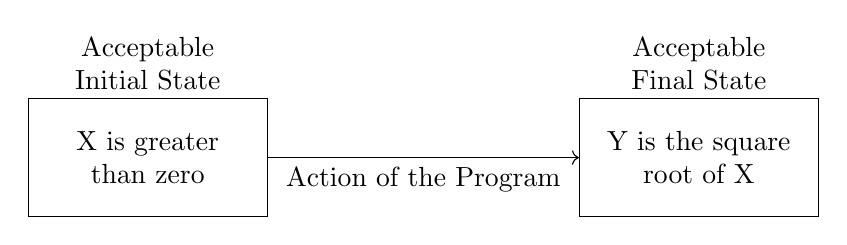
\begin{tikzpicture}
            % Define style for the boxes
            \tikzstyle{statebox} = [draw, rectangle, minimum height=1.5cm, text width=2.8cm, align=center]

            % Nodes for states
            \node [statebox] (initial) at (-1,0) {X is greater than zero};
            \node [statebox] (final) at (6,0) {Y is the square root of X};

            % Labels above the states
            \node [align=center] at (-1,1.2) {Acceptable \\ Initial State};
            \node [align=center] at (6,1.2) {Acceptable \\ Final State};

            % Arrow with label for the program's action
            \draw [->] (initial) -- node[below, align=center] {Action of the Program} (final);
        \end{tikzpicture}
    \end{center}
\end{frame}
% Section 3: Hoare's Notation and Basic Concepts
\section{Hoare's Notation}

\begin{frame}{Hoare's Notation}
    \begin{block}{Historical Context}
        C.A.R. Hoare introduced the following notation called a \textbf{partial correctness specification} for specifying what a program does:
        \begin{center}
            \Large $\hoare{P}{C}{Q}$
        \end{center}
    \end{block}
    
    \begin{block}{Components}
        \begin{itemize}
            \item $C$ is a command (a program or program fragment)
            \item $P$ and $Q$ are conditions on the program variables used in $C$
            \item $P$ is called the \textbf{precondition}
            \item $Q$ is called the \textbf{postcondition}
        \end{itemize}
    \end{block}
\end{frame}

\begin{frame}{The Precondition (P)}
    \begin{block}{Acceptable Initial State}
        The \textbf{precondition} defines the set of initial states for which the program is guaranteed to work correctly.
        \begin{itemize}
            \item It's an assumption about the values of program variables before execution.
            \item If the precondition is not met, the program has no obligations. It can crash, loop forever, or produce a wrong answer.
            \item Note: Reasoning about memory layout and heap requires \emph{Separation Logic}, an extension of Hoare Logic.
        \end{itemize}
    \end{block}

    \begin{example}
        For a program that calculates the square root of X:
        \begin{center}
            Informal: ``X is greater than zero''\\
            Formal: $\pre{X > 0}$
        \end{center}
    \end{example}
\end{frame}

\begin{frame}{The Postcondition (Q)}
    \begin{block}{Acceptable Final State}
        The \textbf{postcondition} describes the state of the program after it has finished executing.
        \begin{itemize}
            \item It's the "promise" or "guarantee" of the specification.
            \item It typically relates the final values of variables to their initial values.
        \end{itemize}
    \end{block}

    \begin{example}
        For the square root program:
        \begin{center}
            Informal: ``Y is the square root of X''\\
            Formal: $\post{Y \times Y = X \wedge Y \ge 0}$
        \end{center}
        (Note: we relate the final value of Y to the initial value of X).
    \end{example}
\end{frame}

\begin{frame}{Writing Conditions}
    \begin{block}{Mathematical Notation}
        Conditions on program variables will be written using standard mathematical notations together with \textbf{logical operators}:
        \begin{itemize}
            \item $\wedge$ (and)
            \item $\vee$ (or)
            \item $\neg$ (not)
            \item $\Rightarrow$ (implies)
        \end{itemize}
    \end{block}
    
    \begin{example}
        Some example conditions:
        \begin{itemize}
            \item $x > 0 \wedge y \geq 0$ (x is positive AND y is non-negative)
            \item $x = 0 \vee y = 0$ (x equals zero OR y equals zero)
            \item $x > 0 \Rightarrow x^2 > 0$ (if x is positive, then x squared is positive)
        \end{itemize}
    \end{example}
\end{frame}

\begin{frame}{Formal Specification: The Hoare Triple}
    \begin{block}{Combining Pre- and Postconditions}
        Hoare Logic provides a formal notation to write specifications, called a \textbf{Hoare Triple}.
        \[ \hoare{P}{S}{Q} \]
        This is read as:
        \begin{quote}
            If the precondition $P$ is true before executing the program $S$, and if $S$ terminates, then the postcondition $Q$ will be true afterward.
        \end{quote}
    \end{block}

    \begin{example}[Square Root Specification]
        Combining our previous examples, the specification for a square root program $S$ is:
        \[ \hoare{X > 0}{S}{Y \times Y = X \wedge Y \ge 0} \]
        Here, $S$ is the placeholder for the actual program code (the "Action").
    \end{example}
\end{frame}

\begin{frame}{Evolution of Notation}
    \begin{block}{Historical Note}
        Hoare's original notation was $P\ \{C\}\ Q$ not $\hoare{P}{C}{Q}$, but the latter form is now more widely used.
    \end{block}
    
    \begin{block}{Alternative Notations}
        You may encounter different notations in the literature:
        \begin{itemize}
            \item Original: $P\ \{C\}\ Q$
            \item Modern: $\hoare{P}{C}{Q}$
            \item Some texts: $\{P\}\ C\ \{Q\}$ (without special formatting)
        \end{itemize}
        All represent the same concept: a partial correctness specification.
    \end{block}
\end{frame}

\begin{frame}{Partial Correctness}
    \begin{block}{What is Partial Correctness?}
        A Hoare triple $\hoare{P}{C}{Q}$ expresses \textbf{partial correctness}:
        \begin{quote}
            \emph{If} the precondition $P$ is true before executing command $C$, \emph{and if} $C$ terminates, \emph{then} the postcondition $Q$ will be true after execution.
        \end{quote}
    \end{block}
    
    \begin{alertblock}{Important: Termination Not Guaranteed}
        Partial correctness does \textbf{not} guarantee that the program terminates!
        \begin{itemize}
            \item It only says what must be true \emph{if} the program terminates
            \item A program that loops forever can still be partially correct
            \item Total correctness = Partial correctness + Termination
        \end{itemize}
    \end{alertblock}
\end{frame}

\begin{frame}{Reading Hoare Triples}
    \begin{block}{How to Read $\hoare{P}{C}{Q}$}
        The triple $\hoare{P}{C}{Q}$ can be read as:
        \begin{enumerate}
            \item ``If $P$ is true, then after $C$ executes, $Q$ will be true''
            \item ``$C$ transforms states satisfying $P$ into states satisfying $Q$''
            \item ``Starting from $P$, command $C$ establishes $Q$''
        \end{enumerate}
    \end{block}
    
    \begin{example}[Simple Assignment]
        $\hoare{x = 5}{\assign{y}{x + 1}}{y = 6}$
        
        This reads as: ``If $x$ equals 5 before the assignment, then $y$ will equal 6 after the assignment.''
    \end{example}
\end{frame}

\begin{frame}{Meaning of Hoare's Notation}
    \begin{block}{Formal Definition}
        $\hoare{P}{C}{Q}$ is true if:
        \begin{itemize}
            \item whenever $C$ is executed in a state satisfying $P$
            \item and \emph{if} the execution of $C$ terminates
            \item then the state in which $C$ terminates satisfies $Q$
        \end{itemize}
    \end{block}
    
    \begin{example}[Assignment Command]
        Consider: $\hoare{X = 1}{X := X + 1}{X = 2}$
        \begin{itemize}
            \item $P$ is the condition that the value of X is 1
            \item $Q$ is the condition that the value of X is 2
            \item $C$ is the assignment command $X := X + 1$ (i.e. `X becomes X+1')
        \end{itemize}
    \end{example}
\end{frame}

\begin{frame}{Truth and Falsity of Hoare Triples}
    \begin{example}[True Triple]
        $\hoare{X = 1}{X := X + 1}{X = 2}$ is \textbf{true}
        
        \textbf{Why?} Starting from a state where $X = 1$, executing $X := X + 1$ results in $X = 2$.
    \end{example}
    
    \begin{example}[False Triple]
        $\hoare{X = 1}{X := X + 1}{X = 3}$ is \textbf{false}
        
        \textbf{Why?} Starting from $X = 1$, executing $X := X + 1$ results in $X = 2$, not $X = 3$.
    \end{example}
    
    \begin{alertblock}{Key Insight}
        A Hoare triple is a mathematical statement that can be either true or false. It makes a claim about what happens when a program executes.
    \end{alertblock}
\end{frame}
% Section 4: Hoare Logic and Verification
\section{Hoare Logic and Verification}

\begin{frame}{Hoare Logic and Verification Conditions}
    \begin{block}{What is Hoare Logic?}
        Hoare Logic is a \textbf{deductive proof system} for Hoare triples $\hoare{P}{C}{Q}$
        \begin{itemize}
            \item Provides \textbf{axioms} (basic facts about simple commands) and \textbf{inference rules} (ways to combine proofs)
            \item Example: Assignment axiom, sequence rule, while loop rule
            \item Forms the theoretical foundation for program verification
        \end{itemize}
    \end{block}
    
    \begin{block}{Direct Verification with Hoare Logic}
        \textbf{Advantages:}
        \begin{itemize}
            \item Original proposal by Hoare
            \item Provides complete formal proofs
        \end{itemize}
        
        \textbf{Disadvantages:}
        \begin{itemize}
            \item Tedious and error-prone for humans
            \item Impractical for large programs
            \item Requires detailed manual proof construction
        \end{itemize}
    \end{block}
\end{frame}

\begin{frame}{Verification Conditions}
    \begin{block}{Definition: What is a Verification Condition?}
        A \textbf{verification condition} is a mathematical formula (without program constructs) whose truth implies the correctness of a program.
        \begin{itemize}
            \item Generated from Hoare triples by analyzing the program structure
            \item Expressed purely in terms of logic and mathematics
            \item No references to program execution or state changes
        \end{itemize}
    \end{block}
\end{frame}

\begin{frame}{Verification Conditions -2}

        \begin{block}{Modern Approach: Verification Conditions}
        Can `compile' proving $\hoare{P}{C}{Q}$ to \textbf{verification conditions}
        \begin{itemize}
            \item More natural for automated reasoning
            \item Basis for computer-assisted verification
            \item Separates program logic from mathematical reasoning
        \end{itemize}
    \end{block}
\end{frame}

\begin{frame}{Verification Conditions -3}
    \begin{block}{Key Property}
        Proof of verification conditions is \textbf{equivalent} to proof with Hoare Logic
        \begin{itemize}
            \item Hoare Logic can be used to \emph{explain} verification conditions
            \item Both approaches prove the same correctness properties
            \item Verification conditions are more amenable to automation
        \end{itemize}
    \end{block}
\end{frame}

\begin{frame}{Verification Condition Example}
    \begin{example}[Simple Verification Condition]
        To prove $\hoare{x > 0}{y := x + 1}{y > 1}$:
        
        \textbf{Step 1:} Analyze what the program does
        \begin{itemize}
            \item The assignment $y := x + 1$ sets $y$ to the value of $x + 1$
        \end{itemize}
        
        \textbf{Step 2:} Generate the verification condition
        \begin{itemize}
            \item We need: if $x > 0$ initially, then $y > 1$ after assignment
            \item Since $y$ will equal $x + 1$, we need: $x > 0 \Rightarrow (x + 1) > 1$
        \end{itemize}
        
        \textbf{Step 3:} The verification condition is:
        \[x > 0 \Rightarrow (x + 1) > 1\]
        
        This is a pure mathematical statement that can be proved using algebra, without any reference to program execution!
    \end{example}
\end{frame}
% Section 5: Partial and Total Correctness
\section{Partial and Total Correctness}

\begin{frame}{Partial Correctness Specification}
    \begin{block}{Definition}
        An expression $\hoare{P}{C}{Q}$ is called a \textbf{partial correctness specification}
        \begin{itemize}
            \item $P$ is called its \textbf{precondition}
            \item $Q$ its \textbf{postcondition}
        \end{itemize}
    \end{block}
    
    \begin{block}{When is $\hoare{P}{C}{Q}$ true?}
        $\hoare{P}{C}{Q}$ is true if:
        \begin{itemize}
            \item whenever $C$ is executed in a state satisfying $P$
            \item and \emph{if} the execution of $C$ terminates
            \item then the state in which $C$'s execution terminates satisfies $Q$
        \end{itemize}
    \end{block}
\end{frame}

\begin{frame}{Why ``Partial'' Correctness?}
    \begin{block}{The Key Point}
        These specifications are `partial' because for $\hoare{P}{C}{Q}$ to be true it is \textbf{not} necessary for the execution of $C$ to terminate when started in a state satisfying $P$
    \end{block}
    
    \begin{block}{What is Required}
        It is only required that \emph{if} the execution terminates, \emph{then} $Q$ holds
    \end{block}
    
    \begin{example}[Infinite Loop]
        $\hoare{X = 1}{\text{WHILE T DO } X := X}{Y = 2}$ -- \colorbox{yellow}{this specification is true!}
        
        \textbf{Why?} The loop never terminates, so we never need to check if $Y = 2$. The specification only makes a claim about what happens \emph{if} the program terminates.
    \end{example}
\end{frame}

\begin{frame}{Total Correctness Specification}
    \begin{block}{Definition}
        A stronger kind of specification is a \textbf{total correctness specification}
        \begin{itemize}
            \item There is no standard notation for such specifications
            \item We shall use $[P]\ C\ [Q]$
        \end{itemize}
    \end{block}
    
    \begin{block}{When is $[P]\ C\ [Q]$ true?}
        A total correctness specification $[P]\ C\ [Q]$ is true if and only if:
        \begin{itemize}
            \item whenever $C$ is executed in a state satisfying $P$ the \colorbox{yellow}{execution of $C$ terminates}
            \item after $C$ terminates $Q$ holds
        \end{itemize}
    \end{block}
\end{frame}

\begin{frame}{Total Correctness Example}
    \begin{example}[False Total Correctness]
        $[X = 1]\ Y := X;\ \text{WHILE T DO } X := X\ [Y = 1]$
        
        This says that:
        \begin{itemize}
            \item the execution of $Y := X;\ \text{WHILE T DO } X := X$ terminates when started in a state satisfying $X = 1$
            \item after which $Y = 1$ will hold
        \end{itemize}
        
        \textbf{This is clearly false} because the while loop never terminates!
    \end{example}
    
    \begin{alertblock}{Key Difference}
        \begin{itemize}
            \item Partial correctness: $\hoare{P}{C}{Q}$ -- ``If it terminates, then...''
            \item Total correctness: $[P]\ C\ [Q]$ -- ``It terminates and then...''
        \end{itemize}
    \end{alertblock}
\end{frame}

\begin{frame}{Relationship Between Partial and Total Correctness}
    \begin{block}{Mathematical Relationship}
        Total correctness = Partial correctness + Termination
        
        \[[P]\ C\ [Q] \equiv \hoare{P}{C}{Q} \wedge \text{``$C$ terminates when started in a state satisfying $P$''}\]
    \end{block}
    
    \begin{block}{Practical Implications}
        \begin{itemize}
            \item Proving partial correctness is often easier
            \item Proving termination requires additional techniques
            \begin{itemize}
                \item \textbf{Variant functions}: expressions that decrease with each loop iteration and are bounded below
                \item Also called \emph{ranking functions} or \emph{termination measures}
            \end{itemize}
            \item Many verification tools focus on partial correctness first
            \item Total correctness is needed for critical systems
        \end{itemize}
    \end{block}
\end{frame}
% Section 6: Auxiliary Variables
\section{Auxiliary Variables}

\begin{frame}{Auxiliary Variables}
    \begin{example}[Variable Swap]
        $\hoare{X=x \wedge Y=y}{R:=X;\ X:=Y;\ Y:=R}{X=y \wedge Y=x}$
        
        This says that \emph{if} the execution of
        \begin{center}
            \texttt{R:=X; X:=Y; Y:=R}
        \end{center}
        terminates (which it does)
        
        \emph{then} the values of X and Y are exchanged
    \end{example}
    
    \begin{block}{Key Observation}
        The variables $x$ and $y$, which don't occur in the command and are used to name the initial values of program variables $X$ and $Y$
    \end{block}
\end{frame}

\begin{frame}{What are Auxiliary Variables?}
    \begin{block}{Definition}
        Variables that appear in specifications but not in the program code are called:
        \begin{itemize}
            \item \textbf{Auxiliary variables}
            \item \textbf{Ghost variables}
            \item \textbf{Specification variables}
        \end{itemize}
    \end{block}
    
    \begin{block}{Purpose}
        Auxiliary variables allow us to:
        \begin{itemize}
            \item Refer to initial values of program variables in postconditions
            \item Express relationships between initial and final states
            \item Write more expressive specifications
        \end{itemize}
    \end{block}
\end{frame}

\begin{frame}{Naming Convention}
    \begin{block}{Informal Convention}
        To distinguish between program variables and auxiliary variables:
        \begin{itemize}
            \item \textbf{Program variables} are UPPER CASE (e.g., X, Y, Z)
            \item \textbf{Auxiliary variables} are lower case (e.g., x, y, z)
        \end{itemize}
    \end{block}
    
    \begin{example}[More Examples]
        \begin{itemize}
            \item $\hoare{X=x}{X:=X+1}{X=x+1}$ -- $x$ remembers initial value
            \item $\hoare{X=x \wedge Y=y}{X:=X+Y}{X=x+y \wedge Y=y}$
            \item $\hoare{A[i]=a}{A[i]:=0}{A[i]=0 \wedge \text{``old } A[i] = a\text{''}}$
        \end{itemize}
    \end{example}
\end{frame}

\begin{frame}{Why Auxiliary Variables Matter}
    \begin{block}{Without Auxiliary Variables}
        Consider trying to specify variable swap without auxiliary variables:
        \begin{itemize}
            \item $\hoare{?}{R:=X;\ X:=Y;\ Y:=R}{?}$
            \item How do we say ``X gets Y's initial value''?
            \item We can't refer to initial values!
        \end{itemize}
    \end{block}
    
    \begin{block}{With Auxiliary Variables}
        We can express complex relationships:
        \begin{itemize}
            \item Maximum: $\hoare{X=x \wedge Y=y}{...}{M = \max(x,y)}$
            \item Sorting: $\hoare{A=a}{...}{\text{``A is a sorted permutation of a''}}$
            \item Any computation relating initial and final states
        \end{itemize}
    \end{block}
\end{frame}

\begin{frame}{Important Notes about Auxiliary Variables}
    \begin{alertblock}{Key Properties}
        \begin{enumerate}
            \item Auxiliary variables are \textbf{immutable} -- they never change value during program execution
            \item They exist only in specifications, not in the actual program
            \item They are universally quantified (implicitly)
        \end{enumerate}
    \end{alertblock}
    
    \begin{block}{Formal Interpretation}
        The specification $\hoare{X=x}{C}{Q(x)}$ actually means:
        \[\forall x.\ \hoare{X=x}{C}{Q(x)}\]
        ``For all values $x$, if $X$ starts with value $x$, then after $C$, property $Q(x)$ holds''
    \end{block}
\end{frame}
% Section 7: Floyd-Hoare Logic
\section{Floyd-Hoare Logic}

\begin{frame}{Floyd-Hoare Logic}
    \begin{block}{The Need for Formal Proofs}
        To construct formal proofs of partial correctness specifications, \emph{axioms} and \emph{rules of inference} are needed
    \end{block}
    
    \begin{block}{What Floyd-Hoare Logic Provides}
        This is what Floyd-Hoare logic provides:
        \begin{itemize}
            \item The formulation of the deductive system is due to Hoare
            \item Some of the underlying ideas originated with Floyd
        \end{itemize}
    \end{block}
\end{frame}

\begin{frame}{Structure of Proofs in Floyd-Hoare Logic}
    \begin{block}{Proof Definition}
        A proof in Floyd-Hoare logic is a sequence of lines, each of which is either:
        \begin{itemize}
            \item An \textbf{axiom} of the logic, or
            \item Follows from earlier lines by a \textbf{rule of inference} of the logic
        \end{itemize}
        
        Note: Proofs can also be trees, if you prefer
    \end{block}
    
    \begin{block}{Purpose of Formal Proofs}
        A formal proof makes explicit what axioms and rules of inference are used to arrive at a conclusion
    \end{block}
\end{frame}

\begin{frame}{Components of Floyd-Hoare Logic}
    \begin{block}{Axioms}
        \textbf{Axioms} are basic facts about specific programming constructs that require no proof:
        \begin{itemize}
            \item Assignment axiom
            \item Skip axiom (for the empty command)
            \item Other basic command axioms
        \end{itemize}
    \end{block}
    
    \begin{block}{Rules of Inference}
        \textbf{Rules of inference} allow us to derive new facts from existing ones:
        \begin{itemize}
            \item Sequence rule (composition)
            \item Conditional rule (if-then-else)
            \item While loop rule
            \item Consequence rule
        \end{itemize}
    \end{block}
\end{frame}

\begin{frame}{Historical Context}
    \begin{block}{Robert W. Floyd (1936-2001)}
        \begin{itemize}
            \item Introduced flowchart-based verification methods (1967)
            \item Pioneered the use of loop invariants
            \item Developed techniques for proving program termination
        \end{itemize}
    \end{block}
    
    \begin{block}{C.A.R. Hoare (1934-)}
        \begin{itemize}
            \item Formalized Floyd's ideas into a logical system (1969)
            \item Introduced the triple notation $\{P\} C \{Q\}$
            \item Created the axiomatic semantics approach
        \end{itemize}
    \end{block}
    
    \begin{alertblock}{Note}
        The system is called ``Floyd-Hoare Logic'' to honor both contributors
    \end{alertblock}
\end{frame}

\begin{frame}{Example: What a Proof Looks Like}
    \begin{example}[Simple Proof Structure]
        To prove $\hoare{x = 5}{y := x + 1; z := y}{z = 6}$:
        
        \begin{enumerate}
            \item $\hoare{x = 5}{y := x + 1}{y = 6}$ \hfill (Assignment axiom)
            \item $\hoare{y = 6}{z := y}{z = 6}$ \hfill (Assignment axiom)
            \item $\hoare{x = 5}{y := x + 1; z := y}{z = 6}$ \hfill (Sequence rule on 1,2)
        \end{enumerate}
        
        Each line is justified by an axiom or rule!
    \end{example}
    
    \begin{block}{Key Insight}
        Floyd-Hoare Logic provides a \emph{systematic} way to prove program correctness, not just intuitive arguments
    \end{block}
\end{frame}
% Section 8: Judgements
\section{Judgements}

\begin{frame}{Judgements}
    \begin{block}{Three Kinds of Things That Could Be True or False}
        \begin{itemize}
            \item \textbf{Statements of mathematics}, e.g., $(X + 1)^2 = X^2 + 2 \times X + 1$
            \item \textbf{Partial correctness specifications} $\{P\} C \{Q\}$
            \item \textbf{Total correctness specifications} $[P] C [Q]$
        \end{itemize}
    \end{block}
    
    \begin{block}{What Are Judgements?}
        These three kinds of things are examples of \emph{judgements}
        \begin{itemize}
            \item A logical system gives rules for proving judgements
            \item Floyd-Hoare logic provides rules for proving partial correctness specifications
            \item The laws of arithmetic provide ways of proving statements about integers
        \end{itemize}
    \end{block}
\end{frame}

\begin{frame}{Proving Judgements}
    \begin{block}{The Turnstile Notation}
        $\vdash S$ means statement $S$ can be proved
        \begin{itemize}
            \item How to prove predicate calculus statements assumed known
            \item This course covers axioms and rules for proving \emph{program correctness statements}
        \end{itemize}
    \end{block}
    
    \begin{alertblock}{Note}
        We will introduce the specific axioms and inference rules of Floyd-Hoare logic in detail in the following sections
    \end{alertblock}
    
    \begin{example}[Different Types of Provable Judgements]
        \begin{itemize}
            \item $\vdash (x + y)^2 = x^2 + 2xy + y^2$ (mathematical)
            \item $\vdash \{x = 5\} y := x + 1 \{y = 6\}$ (program correctness)
            \item $\vdash [x \geq 0] y := \sqrt{x} [y^2 = x]$ (total correctness)
        \end{itemize}
    \end{example}
\end{frame}

\begin{frame}{Why Judgements Matter}
    \begin{block}{Formal vs Informal Reasoning}
        \begin{itemize}
            \item \textbf{Informal}: ``Obviously, if x=5 then after y:=x+1, y will be 6''
            \item \textbf{Formal}: Use axioms and rules to derive $\vdash \{x = 5\} y := x + 1 \{y = 6\}$
        \end{itemize}
    \end{block}
    
    \begin{block}{Benefits of Formal Judgements}
        \begin{enumerate}
            \item \textbf{Precision}: No ambiguity about what needs to be proved
            \item \textbf{Mechanization}: Can be checked by computers
            \item \textbf{Composability}: Complex proofs built from simpler ones
            \item \textbf{Confidence}: Mathematical certainty about correctness
        \end{enumerate}
    \end{block}
\end{frame}

\begin{frame}{Types of Logical Systems}
    \begin{block}{Different Logical Systems for Different Judgements}
        \begin{tabular}{|l|l|}
            \hline
            \textbf{Judgement Type} & \textbf{Logical System} \\
            \hline
            Mathematical statements & Predicate logic, arithmetic \\
            Partial correctness & Floyd-Hoare logic \\
            Total correctness & Extended Hoare logic \\
            Type checking & Type systems \\
            \hline
        \end{tabular}
    \end{block}
    
    \begin{block}{Focus of This Course}
        This course focuses on Floyd-Hoare logic for proving partial correctness specifications
        \begin{itemize}
            \item We'll learn the axioms (basic facts)
            \item We'll learn the inference rules (ways to combine facts)
            \item We'll practice constructing formal proofs
        \end{itemize}
    \end{block}
\end{frame}
% Section 9: Language and Substitution
\section{Foundations for Axioms and Rules}

\begin{frame}{Reminder of our Little Programming Language}
    \begin{block}{Axiomatic Semantics}
        The proof rules that follow constitute an \emph{axiomatic semantics} of our programming language
    \end{block}

    \begin{block}{Expressions}
        \[ E ::= N \mid V \mid E_1 + E_2 \mid E_1 - E_2 \mid E_1 \times E_2 \mid \ldots \]
    \end{block}

    \begin{block}{Boolean expressions}
        \[ B ::= \mathbf{T} \mid \mathbf{F} \mid E_1 = E_2 \mid E_1 \leq E_2 \mid \ldots \]
    \end{block}


\end{frame}

\begin{frame}{Reminder of our Little Programming Language - 2}
    \begin{block}{Commands}
        \begin{align*}
            C ::= & \quad V := E & \text{Assignments} \\
            & \mid C_1 ; C_2 & \text{Sequences} \\
            & \mid \text{IF } B \text{ THEN } C_1 \text{ ELSE } C_2 & \text{Conditionals} \\
            & \mid \text{WHILE } B \text{ DO } C & \text{WHILE-commands}
        \end{align*}
    \end{block}
\end{frame}

\begin{frame}{Substitution Notation}
    \begin{block}{Definition}
        $Q[E/V]$ is the result of replacing all occurrences of $V$ in $Q$ by $E$
        \begin{itemize}
            \item Read $Q[E/V]$ as `$Q$ with $E$ for $V$'
            \item For example: $(X+1 > X)[Y+Z/X] = ((Y+Z)+1 > Y+Z)$
            \item Ignoring issues with bound variables for now (e.g. variable capture)
        \end{itemize}
    \end{block}

    \begin{block}{Substitution in Terms}
        Same notation for substituting into terms, e.g. $E_1[E_2/V]$
    \end{block}
\end{frame}

\begin{frame}{The Cancellation Law}
    \begin{block}{Substitution as Cancellation}
        Think of this notation as the `cancellation law'
        \[ V[E/V] = E \]
        which is analogous to the cancellation property of fractions
        \[ v \times (e/v) = e \]
    \end{block}

    \begin{alertblock}{Important Property}
        Note that $Q[x/V]$ doesn't contain $V$ (if $V \neq x$)
    \end{alertblock}

\end{frame}

\begin{frame}{The Cancellation Law - 2}
    \begin{example}[Substitution Examples]
        \begin{itemize}
            \item $(X + Y > 0)[5/X] = (5 + Y > 0)$
            \item $(X \times X = Y)[X+1/X] = ((X+1) \times (X+1) = Y)$
            \item $(X > Y \wedge Y > Z)[W/Y] = (X > W \wedge W > Z)$
        \end{itemize}
    \end{example}
\end{frame}

\begin{frame}{Why Substitution Matters}
    \begin{block}{Connection to Assignment}
        Substitution notation is crucial for understanding the assignment axiom:
        \begin{itemize}
            \item If we want $Q$ to be true after $V := E$
            \item Then $Q[E/V]$ must be true before
            \item Because after assignment, $V$ will have the value that $E$ had before
        \end{itemize}
    \end{block}

    \begin{block}{Preview: Assignment Axiom}
        This leads to the assignment axiom (details coming next)
    \end{block}
\end{frame}

\begin{frame}{Reading Inference Rules}
    \begin{block}{Inference Rule Notation}
        Before we see the axioms and rules, let's understand the notation:
        \[ \frac{\text{premises}}{\text{conclusion}} \]
        \begin{itemize}
            \item The line is read as ``implies'' or ``allows us to derive''
            \item Above the line: what we need to prove (premises)
            \item Below the line: what we can conclude
            \item If nothing above the line: it's an \textbf{axiom} (needs no proof)
        \end{itemize}
    \end{block}
    
\end{frame}

\begin{frame}{Reading Inference Rules - 2}
    \begin{example}[Reading an Inference Rule]
        \[ \frac{A \quad B}{C} \]
        This means: ``If we can prove $A$ and we can prove $B$, then we can conclude $C$''
    \end{example}
\end{frame}

\begin{frame}{The Assignment Axiom}
    \begin{block}{Assignment Axiom}
        Now we can understand the assignment axiom:
        \[ \frac{}{\{Q[E/V]\} \; V := E \; \{Q\}} \]
        \begin{itemize}
            \item Nothing above the line = this is an axiom
            \item Below the line = what we can always conclude
            \item Read: ``We can always derive that $\{Q[E/V]\} \; V := E \; \{Q\}$ is true''
        \end{itemize}
    \end{block}
    
    \begin{block}{Understanding the Axiom}
        Read backwards: to achieve $Q$ after $V := E$, need $Q[E/V]$ before
    \end{block}
\end{frame}

\begin{frame}{The Assignment Axiom (Hoare)}
    \begin{block}{Assignment Syntax and Semantics}
        \begin{itemize}
            \item \textbf{Syntax}: $V := E$
            \item \textbf{Semantics}: value of $V$ in final state is value of $E$ in initial state
            \item \textbf{Example}: $X := X + 1$ (adds one to the value of the variable $X$)
        \end{itemize}
    \end{block}
    
    \begin{block}{The Assignment Axiom}
        \[ \vdash \{Q[E/V]\} \; V := E \; \{Q\} \]
        Where $V$ is any variable, $E$ is any expression, $Q$ is any statement.
    \end{block}
\end{frame}

\begin{frame}{Instances of the Assignment Axiom}
    \begin{block}{Examples}
        Instances of the assignment axiom are:
        \begin{itemize}
            \item $\vdash \{E = x\} \; V := E \; \{V = x\}$
            \item $\vdash \{Y = 2\} \; X := 2 \; \{Y = X\}$
            \item $\vdash \{X + 1 = n + 1\} \; X := X + 1 \; \{X = n + 1\}$
            \item $\vdash \{E = E\} \; X := E \; \{X = E\}$ (if $X$ does not occur in $E$)
        \end{itemize}
    \end{block}
    
    \begin{block}{Key Insight}
        The precondition is obtained by substituting $E$ for $V$ in the postcondition!
    \end{block}
\end{frame}

\begin{frame}{Understanding the Assignment Axiom}
    \begin{block}{Why Does This Work?}
        Let's think step by step:
        \begin{enumerate}
            \item We want property $Q$ to hold after executing $V := E$
            \item After the assignment, $V$ has the value that $E$ had before
            \item So if we want $Q$ to be true about $V$ after...
            \item Then $Q$ must have been true about $E$ before!
            \item That's exactly what $Q[E/V]$ expresses
        \end{enumerate}
    \end{block}
    
    \begin{example}[Step-by-Step]
        Want: $\{?\} \; X := Y + 1 \; \{X > 5\}$
        \begin{itemize}
            \item After: $X > 5$ must be true
            \item Before: $(Y + 1) > 5$ must be true
            \item So: $\{Y + 1 > 5\} \; X := Y + 1 \; \{X > 5\}$
        \end{itemize}
    \end{example}
\end{frame}

\begin{frame}{The Backwards Fallacy}
    \begin{block}{Common Misconception}
        Many people feel the assignment axiom is `backwards'
    \end{block}
    
    \begin{block}{First Erroneous Intuition}
        One common erroneous intuition is that it should be:
        \[ \vdash \{P\} \; V := E \; \{P[V/E]\} \]
        where $P[V/E]$ denotes the result of substituting $V$ for $E$ in $P$
    \end{block}
    
    \begin{alertblock}{Why This is Wrong}
        This has the false consequence $\vdash \{X = 0\} \; X := 1 \; \{X = 0\}$
        \begin{itemize}
            \item Since $(X = 0)[X/1]$ is equal to $(X = 0)$ 
            \item Because $1$ doesn't occur in $(X = 0)$
            \item But clearly $X$ cannot equal $0$ after we set it to $1$!
        \end{itemize}
    \end{alertblock}
\end{frame}

\begin{frame}{The Backwards Fallacy - 2}
    \begin{block}{Second Erroneous Intuition}
        Another erroneous intuition is that it should be:
        \[ \vdash \{P\} \; V := E \; \{P[E/V]\} \]
    \end{block}
    
    \begin{alertblock}{Why This is Also Wrong}
        This has the false consequence $\vdash \{X = 0\} \; X := 1 \; \{1 = 0\}$
        \begin{itemize}
            \item Taking $P$ to be $X = 0$, $V$ to be $X$, and $E$ to be $1$
            \item We get $(X = 0)[1/X] = (1 = 0)$
            \item But $1 = 0$ is always false!
        \end{itemize}
    \end{alertblock}
    
    \begin{block}{The Correct Direction}
        The assignment axiom goes ``backwards'' because we substitute in the \emph{precondition}, not the postcondition!
    \end{block}
\end{frame}

\begin{frame}{Why ``Backwards'' is Actually Forward}
    \begin{block}{Think About Information Flow}
        The assignment axiom seems backwards but it's actually forward-thinking:
        \begin{itemize}
            \item We start with what we \emph{want} (the postcondition $Q$)
            \item We work out what we \emph{need} (the precondition $Q[E/V]$)
            \item This is called \textbf{weakest precondition reasoning}
        \end{itemize}
    \end{block}
    
    \begin{example}[Working Backwards]
        Goal: Ensure $Y = 10$ after $Y := X \times 2$
        \begin{itemize}
            \item Postcondition: $Y = 10$
            \item Substitute: $(Y = 10)[X \times 2/Y] = (X \times 2 = 10)$
            \item Simplify: $X = 5$
            \item Result: $\{X = 5\} \; Y := X \times 2 \; \{Y = 10\}$
        \end{itemize}
    \end{example}
\end{frame}

\section{Validity and Limitations of the Assignment Axiom}

\begin{frame}{Validity}
    \begin{block}{The Importance of Validity}
        Important to establish the validity of axioms and rules
    \end{block}
    
    \begin{block}{Formal Semantics and Soundness}
        Later will give a \emph{formal semantics} of our little programming language
        \begin{itemize}
            \item Then \emph{prove} axioms and rules of inference of Floyd-Hoare logic are sound
            \item This will only increase our confidence in the axioms and rules to the extent that we believe the correctness of the formal semantics!
        \end{itemize}
    \end{block}
\end{frame}

\begin{frame}{The Assignment Axiom in Real Languages}
    \begin{alertblock}{Important Limitation}
        The Assignment Axiom is not valid for `real' programming languages
    \end{alertblock}
    
    \begin{block}{Historical Note}
        In an early PhD on Hoare Logic, G. Ligler showed that the assignment axiom can fail to hold in six different ways for the language Algol 60
    \end{block}
    
    \begin{block}{Why This Matters}
        \begin{itemize}
            \item Our simple language has carefully chosen features
            \item Real languages have complications that break the axiom
            \item Understanding these limitations helps us apply Hoare Logic correctly
        \end{itemize}
    \end{block}
\end{frame}

\begin{frame}{Expressions with Side Effects}
    \begin{block}{The Hidden Assumption}
        The validity of the assignment axiom depends on expressions not having side effects
    \end{block}
    
    \begin{example}[Block Expression]
        Suppose our language were extended to contain the `block expression':
        \begin{center}
            \texttt{BEGIN Y:=1; 2 END}
        \end{center}
        \begin{itemize}
            \item This expression has value 2
            \item But its evaluation also `side effects' the variable Y by storing 1 in it
        \end{itemize}
    \end{example}
\end{frame}

\begin{frame}{Why Side Effects Break the Assignment Axiom}
    \begin{block}{The Problem}
        If the assignment axiom applied to block expressions, then it could be used to deduce:
        \[ \vdash \{Y=0\} \; X := \texttt{BEGIN Y:=1; 2 END} \; \{Y=0\} \]
    \end{block}
    
    \begin{block}{The Faulty Reasoning}
        \begin{itemize}
            \item Since $(Y=0)[E/X] = (Y=0)$ (because X does not occur in $(Y=0)$)
            \item By the assignment axiom, we'd conclude the above
            \item This is clearly false: after the assignment Y will have the value 1!
        \end{itemize}
    \end{block}
    
    \begin{alertblock}{The Lesson}
        The assignment axiom only works when expressions are \textbf{pure} (no side effects)
    \end{alertblock}
\end{frame}

\begin{frame}{Other Ways the Assignment Axiom Can Fail}
    \begin{block}{Real Language Complications}
        In real programming languages, the assignment axiom can fail due to:
        \begin{enumerate}
            \item \textbf{Side effects in expressions} (as we just saw)
            \item \textbf{Aliasing}: multiple names for the same location
            \item \textbf{Call by reference}: procedure parameters that modify variables
            \item \textbf{Global variables}: hidden dependencies between parts of code
            \item \textbf{Undefined behavior}: division by zero, array bounds violations
            \item \textbf{Concurrent modification}: other threads changing variables
        \end{enumerate}
    \end{block}
    
    \begin{block}{Defensive Programming}
        Understanding these limitations helps us:
        \begin{itemize}
            \item Design better programming languages
            \item Write more verifiable code
            \item Know when we can trust our formal proofs
        \end{itemize}
    \end{block}
\end{frame}

\begin{frame}{Example: Aliasing Breaking the Assignment Axiom}
    \begin{example}[Aliasing Problem]
        Consider if our language had arrays and we tried:
        \[ \vdash \{A[i] = 5\} \; A[j] := 0 \; \{A[i] = 5\} \]
        
        The assignment axiom would suggest this is valid because:
        \begin{itemize}
            \item $(A[i] = 5)[0/A[j]]$ might seem to be just $(A[i] = 5)$
            \item But what if $i = j$? Then $A[i]$ and $A[j]$ are the same location!
            \item After the assignment, $A[i] = 0$, not 5
        \end{itemize}
    \end{example}
    
    \begin{block}{The Solution}
        In real verification:
        \begin{itemize}
            \item Must track when different expressions might refer to same location
            \item Need more sophisticated rules for arrays and pointers
            \item This leads to \emph{separation logic} and other advanced techniques
        \end{itemize}
    \end{block}
\end{frame}

\begin{frame}{A Forwards Assignment Axiom (Floyd)}
    \begin{block}{Floyd's Original Formulation}
        This is the original semantics of assignment due to Floyd:
        \[ \vdash \{P\} \; V := E \; \{\exists v. \; V = E[v/V] \wedge P[v/V]\} \]
        where $v$ is a new variable (i.e., doesn't equal $V$ or occur in $P$ or $E$)
    \end{block}
    
    \begin{block}{What This Means}
        \begin{itemize}
            \item We start with precondition $P$
            \item After assignment, $V$ has the value that $E$ had (with old $V$ replaced by $v$)
            \item The old properties still hold (with old $V$ replaced by $v$)
            \item We use existential quantification to ``remember'' the old value
        \end{itemize}
    \end{block}
\end{frame}

\begin{frame}{Example of the Forwards Axiom}
    \begin{example}[Forwards Assignment]
        \[ \vdash \{X=1\} \; X := X+1 \; \{\exists v. \; X = X+1[v/X] \wedge X=1[v/X]\} \]
    \end{example}
    
    \begin{block}{Simplifying the Postcondition}
        \begin{align*}
            & \vdash \{X=1\} \; X := X+1 \; \{\exists v. \; X = X+1[v/X] \wedge X=1[v/X]\} \\
            & \vdash \{X=1\} \; X := X+1 \; \{\exists v. \; X = v + 1 \wedge v = 1\} \\
            & \vdash \{X=1\} \; X := X+1 \; \{\exists v. \; X = 1 + 1 \wedge v = 1\} \\
            & \vdash \{X=1\} \; X := X+1 \; \{X = 1 + 1 \wedge \exists v. \; v = 1\} \\
            & \vdash \{X=1\} \; X := X+1 \; \{X = 2 \wedge \mathbf{T}\} \\
            & \vdash \{X=1\} \; X := X+1 \; \{X = 2\}
        \end{align*}
    \end{block}
\end{frame}

\begin{frame}{Comparing Forward and Backward Axioms}
    \begin{block}{Key Observation}
        The forwards axiom is equivalent to the standard (backwards) one but harder to use
    \end{block}
    
    \begin{columns}
        \begin{column}{0.48\textwidth}
            \begin{block}{Backwards (Hoare)}
                \[ \vdash \{Q[E/V]\} \; V := E \; \{Q\} \]
                \begin{itemize}
                    \item Direct: substitute in precondition
                    \item Natural for verification
                    \item No existential quantifiers
                \end{itemize}
            \end{block}
        \end{column}
        \begin{column}{0.48\textwidth}
            \begin{block}{Forwards (Floyd)}
                \[ \vdash \{P\} \; V := E \; \{\exists v. \; V = E[v/V] \wedge P[v/V]\} \]
                \begin{itemize}
                    \item Requires existential elimination
                    \item More complex postconditions
                    \item Natural for symbolic execution
                \end{itemize}
            \end{block}
        \end{column}
    \end{columns}
\end{frame}

\begin{frame}{Why Have Two Forms?}
    \begin{block}{Different Use Cases}
        \begin{itemize}
            \item \textbf{Backwards (Hoare)}: Better for \emph{verification}
                \begin{itemize}
                    \item Start with desired postcondition
                    \item Work backwards to find required precondition
                    \item Natural for proving programs meet specifications
                \end{itemize}
            \item \textbf{Forwards (Floyd)}: Better for \emph{analysis}
                \begin{itemize}
                    \item Start with known precondition
                    \item Work forwards to compute postcondition
                    \item Natural for symbolic execution and program analysis
                \end{itemize}
        \end{itemize}
    \end{block}
    
    \begin{block}{In Practice}
        Most verification systems use Hoare's backwards form because:
        \begin{itemize}
            \item Simpler to work with (no existential quantifiers)
            \item More direct for common verification tasks
            \item Easier to automate
        \end{itemize}
    \end{block}
\end{frame}
% Section 11: Rules of Consequence
\section{Rules of Consequence}

\begin{frame}{Precondition Strengthening}
    \begin{block}{Recall}
        Recall that
        \[ \frac{\vdash S_1, \ldots, \vdash S_n}{\vdash S} \]
        means $\vdash S$ can be deduced from $\vdash S_1, \ldots, \vdash S_n$
    \end{block}

\end{frame}

\begin{frame}{Precondition Strengthening}
    \begin{block}{The Rule}
        Using this notation, the rule of \textbf{precondition strengthening} is:
        \[ \frac{\vdash P \Rightarrow P', \quad \vdash \{P'\} \; C \; \{Q\}}{\vdash \{P\} \; C \; \{Q\}} \]
    \end{block}
    \begin{alertblock}{Note}
        The two hypotheses are different kinds of judgements:
        \begin{itemize}
            \item $\vdash P \Rightarrow P'$ is a mathematical/logical judgement
            \item $\vdash \{P'\} \; C \; \{Q\}$ is a program correctness judgement
        \end{itemize}
    \end{alertblock}
\end{frame}

\begin{frame}{Understanding Precondition Strengthening}
    \begin{block}{What Does This Rule Mean?}
        \begin{itemize}
            \item If $P$ implies $P'$ (i.e., $P$ is stronger than $P'$)
            \item And we know that $\{P'\} \; C \; \{Q\}$ holds
            \item Then $\{P\} \; C \; \{Q\}$ also holds
        \end{itemize}
    \end{block}

    \begin{block}{Intuition}
        \begin{itemize}
            \item A stronger precondition gives us more information
            \item If the program works correctly with less information ($P'$)
            \item It will certainly work with more information ($P$)
            \item ``Demanding more from the input never hurts''
        \end{itemize}
    \end{block}


\end{frame}
\begin{frame}{Understanding Precondition Strengthening}
    \begin{example}[Simple Example]
        \begin{itemize}
            \item Know: $\vdash \{x > 0\} \; y := x \; \{y > 0\}$
            \item Have: $x = 5 \Rightarrow x > 0$
            \item Conclude: $\vdash \{x = 5\} \; y := x \; \{y > 0\}$
        \end{itemize}
    \end{example}
\end{frame}

\begin{frame}{Postcondition Weakening}
    \begin{block}{The Dual Rule}
        Just as the previous rule allows the precondition of a partial correctness specification to be strengthened, the following one allows us to weaken the postcondition
    \end{block}

    \begin{block}{Postcondition Weakening Rule}
        \[ \frac{\vdash \{P\} \; C \; \{Q'\}, \quad \vdash Q' \Rightarrow Q}{\vdash \{P\} \; C \; \{Q\}} \]
    \end{block}
\end{frame}

\begin{frame}{Understanding Postcondition Weakening}
    \begin{block}{What Does This Rule Mean?}
        \begin{itemize}
            \item If we can establish $\{P\} \; C \; \{Q'\}$
            \item And $Q'$ implies $Q$ (i.e., $Q'$ is stronger than $Q$)
            \item Then $\{P\} \; C \; \{Q\}$ also holds
        \end{itemize}
    \end{block}

    \begin{block}{Intuition}
        \begin{itemize}
            \item If the program establishes a strong property ($Q'$)
            \item It automatically establishes any weaker property ($Q$)
            \item ``Promising less in the output is always safe''
        \end{itemize}
    \end{block}

    \begin{example}[Simple Example]
        \begin{itemize}
            \item Know: $\vdash \{x = 5\} \; y := x + 1 \; \{y = 6\}$
            \item Have: $y = 6 \Rightarrow y > 0$
            \item Conclude: $\vdash \{x = 5\} \; y := x + 1 \; \{y > 0\}$
        \end{itemize}
    \end{example}
\end{frame}

\begin{frame}{The Rule of Consequence}
    \begin{block}{Combining Both Rules}
        Often we use both precondition strengthening and postcondition weakening together. This gives us the general \textbf{rule of consequence}:

        \[ \frac{\vdash P \Rightarrow P', \quad \vdash \{P'\} \; C \; \{Q'\}, \quad \vdash Q' \Rightarrow Q}{\vdash \{P\} \; C \; \{Q\}} \]
    \end{block}

    \begin{block}{When to Use}
        This rule is essential for:
        \begin{itemize}
            \item Adapting existing proofs to new situations
            \item Simplifying complex preconditions or postconditions
            \item Connecting different parts of a larger proof
        \end{itemize}
    \end{block}
\end{frame}

\begin{frame}{Example: Using the Rule of Consequence}
    \begin{example}[Complete Example]
        Want to prove: $\vdash \{x = 10 \wedge y = 5\} \; z := x - y \; \{z > 0\}$

        \begin{enumerate}
            \item By assignment axiom:
            \[\vdash \{x - y > 0\} \; z := x - y \; \{z > 0\}\]

            \item We need to show: $x = 10 \wedge y = 5 \Rightarrow x - y > 0$
            \begin{itemize}
                \item If $x = 10$ and $y = 5$, then $x - y = 5$
                \item And $5 > 0$ is true
            \end{itemize}

            \item By precondition strengthening:
            \[\vdash \{x = 10 \wedge y = 5\} \; z := x - y \; \{z > 0\}\]
        \end{enumerate}
    \end{example}
\end{frame}

\begin{frame}{Why These Rules Matter}
    \begin{block}{Practical Importance}
        The rules of consequence are crucial because:
        \begin{itemize}
            \item Real programs rarely have specifications that match axioms exactly
            \item We need to adapt and combine different proof rules
            \item They allow modular reasoning about programs
        \end{itemize}
    \end{block}

    \begin{block}{Key Insight}
        These rules formalize the intuition that:
        \begin{itemize}
            \item \textbf{Preconditions}: ``If it works with less, it works with more''
            \item \textbf{Postconditions}: ``If it achieves more, it achieves less''
        \end{itemize}
    \end{block}
\end{frame}
\begin{frame}{Why These Rules Matter}

    \begin{alertblock}{Remember}
        The direction matters:
        \begin{itemize}
            \item Preconditions can be \emph{strengthened} (made more specific)
            \item Postconditions can be \emph{weakened} (made more general)
        \end{itemize}
    \end{alertblock}
\end{frame}
% Section 12: Formal Proofs and Sequencing
\section{Formal Proofs and the Sequencing Rule}

\begin{frame}{An Example Formal Proof}
    \begin{block}{A Little Formal Proof}
        Here is a little formal proof:
    \end{block}
    
    \begin{enumerate}
        \item $\vdash \{R=X \wedge 0=0\} \; Q:=0 \; \{R=X \wedge Q=0\}$ \hfill By the assignment axiom
        \item $\vdash R=X \Rightarrow R=X \wedge 0=0$ \hfill By pure logic
        \item $\vdash \{R=X\} \; Q:=0 \; \{R=X \wedge Q=0\}$ \hfill By precondition strengthening
        \item $\vdash R=X \wedge Q=0 \Rightarrow R=X+(Y \times Q)$ \hfill By laws of arithmetic
        \item $\vdash \{R=X\} \; Q:=0 \; \{R=X+(Y \times Q)\}$ \hfill By postcondition weakening
    \end{enumerate}
    
    \begin{block}{Note}
        The rules precondition strengthening and postcondition weakening are sometimes called the \emph{rules of consequence}
    \end{block}
\end{frame}

\begin{frame}{Analyzing the Example Proof}
    \begin{block}{What This Proof Shows}
        We proved: $\vdash \{R=X\} \; Q:=0 \; \{R=X+(Y \times Q)\}$
        \begin{itemize}
            \item Starting with $R = X$
            \item After setting $Q$ to $0$
            \item We have $R = X + (Y \times 0) = X$
        \end{itemize}
    \end{block}
    
    \begin{block}{Key Steps}
        \begin{enumerate}
            \item Started with assignment axiom for $Q := 0$
            \item Strengthened precondition from $R=X \wedge 0=0$ to just $R=X$
            \item Weakened postcondition using arithmetic ($Y \times 0 = 0$)
        \end{enumerate}
    \end{block}
    
    \begin{block}{Lesson}
        Even simple proofs often require the rules of consequence to connect axioms with desired specifications
    \end{block}
\end{frame}

\begin{frame}{The Sequencing Rule}
    \begin{block}{Syntax and Semantics}
        \begin{itemize}
            \item \textbf{Syntax}: $C_1; \cdots; C_n$
            \item \textbf{Semantics}: the commands $C_1, \cdots, C_n$ are executed in that order
            \item \textbf{Example}: $R:=X; \; X:=Y; \; Y:=R$
            \begin{itemize}
                \item The values of $X$ and $Y$ are swapped using $R$ as a temporary variable
                \item Note \emph{side effect}: value of $R$ changed to the old value of $X$
            \end{itemize}
        \end{itemize}
    \end{block}
    
    \begin{block}{The Sequencing Rule}
        \[ \frac{\vdash \{P\} \; C_1 \; \{Q\}, \quad \vdash \{Q\} \; C_2 \; \{R\}}{\vdash \{P\} \; C_1; C_2 \; \{R\}} \]
    \end{block}
\end{frame}

\begin{frame}{Understanding the Sequencing Rule}
    \begin{block}{What the Rule Says}
        \begin{itemize}
            \item If $C_1$ transforms state from $P$ to $Q$
            \item And $C_2$ transforms state from $Q$ to $R$
            \item Then $C_1; C_2$ transforms state from $P$ to $R$
        \end{itemize}
    \end{block}
    
    \begin{block}{The Middle Condition}
        \begin{itemize}
            \item $Q$ acts as a ``glue'' between the two commands
            \item It must be the postcondition of $C_1$
            \item And the precondition of $C_2$
            \item Finding the right $Q$ is often the key to sequencing proofs
        \end{itemize}
    \end{block}
    
    \begin{block}{Generalization}
        For $n$ commands: need $n-1$ intermediate conditions
        \[ \{P\} \; C_1 \; \{Q_1\} \; C_2 \; \{Q_2\} \; \cdots \; C_{n-1} \; \{Q_{n-1}\} \; C_n \; \{R\} \]
    \end{block}
\end{frame}

\begin{frame}{Example Proof: Variable Swap}
    \begin{block}{Goal}
        Prove the variable swap works correctly
    \end{block}
    
    Example: By the assignment axiom:
    \begin{align*}
        \text{(i)} \quad & \vdash \{X=x \wedge Y=y\} \; R:=X \; \{R=x \wedge Y=y\} \\
        \text{(ii)} \quad & \vdash \{R=x \wedge Y=y\} \; X:=Y \; \{R=x \wedge X=y\} \\
        \text{(iii)} \quad & \vdash \{R=x \wedge X=y\} \; Y:=R \; \{Y=x \wedge X=y\}
    \end{align*}
    
    Hence by (i), (ii) and the sequencing rule:
    \begin{align*}
        \text{(iv)} \quad & \vdash \{X=x \wedge Y=y\} \; R:=X; \; X:=Y \; \{R=x \wedge X=y\}
    \end{align*}
    
    Hence by (iv) and (iii) and the sequencing rule:
    \begin{align*}
        \text{(v)} \quad & \vdash \{X=x \wedge Y=y\} \; R:=X; \; X:=Y; \; Y:=R \; \{Y=x \wedge X=y\}
    \end{align*}
\end{frame}

\begin{frame}{Breaking Down the Swap Proof}
    \begin{block}{Step-by-Step Analysis}
        Starting with $X=x$ and $Y=y$:
        \begin{enumerate}
            \item After $R:=X$: we have $R=x$, $X=x$, $Y=y$
            \item After $X:=Y$: we have $R=x$, $X=y$, $Y=y$ 
            \item After $Y:=R$: we have $R=x$, $X=y$, $Y=x$
        \end{enumerate}
        Final result: $X$ and $Y$ are swapped!
    \end{block}
    
    \begin{block}{Key Observation}
        \begin{itemize}
            \item Each intermediate assertion captures the exact state
            \item We track all variables, including the temporary $R$
            \item The proof is compositional: we prove each step separately
        \end{itemize}
    \end{block}
    
    \begin{alertblock}{Note on Auxiliary Variables}
        The lowercase $x$ and $y$ are auxiliary variables that remember the initial values
    \end{alertblock}
\end{frame}

\begin{frame}{Conditionals}
    \begin{block}{Syntax and Semantics}
        \begin{itemize}
            \item \textbf{Syntax}: \texttt{IF } $S$ \texttt{ THEN } $C_1$ \texttt{ ELSE } $C_2$
            \item \textbf{Semantics}:
            \begin{itemize}
                \item If the statement $S$ is true in the current state, then $C_1$ is executed
                \item If $S$ is false, then $C_2$ is executed
            \end{itemize}
            \item \textbf{Example}: \texttt{IF X<Y THEN MAX:=Y ELSE MAX:=X}
            \begin{itemize}
                \item The value of the variable MAX is set to the maximum of the values of X and Y
            \end{itemize}
        \end{itemize}
    \end{block}
\end{frame}

\begin{frame}{The Conditional Rule}
    \begin{block}{The Conditional Rule}
        \[ \frac{\vdash \{P \wedge S\} \; C_1 \; \{Q\}, \quad \vdash \{P \wedge \neg S\} \; C_2 \; \{Q\}}{\vdash \{P\} \; \texttt{IF } S \texttt{ THEN } C_1 \texttt{ ELSE } C_2 \; \{Q\}} \]
    \end{block}
    
    \begin{block}{Understanding the Rule}
        \begin{itemize}
            \item We need to prove two things:
            \begin{itemize}
                \item When $S$ is true, $C_1$ transforms $P \wedge S$ to $Q$
                \item When $S$ is false, $C_2$ transforms $P \wedge \neg S$ to $Q$
            \end{itemize}
            \item Both branches must establish the same postcondition $Q$
            \item The precondition $P$ is strengthened by the branch condition
        \end{itemize}
    \end{block}
\end{frame}

\begin{frame}{Example: Finding the Maximum}
    \begin{block}{Goal}
        Prove: $\vdash \{\mathbf{T}\} \; \texttt{IF X$\geq$Y THEN MAX:=X ELSE MAX:=Y} \; \{MAX=\max(X,Y)\}$
    \end{block}
\end{frame}
\begin{frame}{Example: Finding the Maximum}

    \begin{block}{Step 1: Logical Facts}
        From Assignment Axiom + Precondition Strengthening:
        \begin{itemize}
            \item $\vdash (X \geq Y \Rightarrow X = \max(X,Y)) \wedge (\neg(X \geq Y) \Rightarrow Y = \max(X,Y))$
        \end{itemize}
    \end{block}
    
    \begin{block}{Step 2: Prove Each Branch}
        It follows that:
        \begin{itemize}
            \item $\vdash \{\mathbf{T} \wedge X \geq Y\} \; MAX:=X \; \{MAX=\max(X,Y)\}$
            \item $\vdash \{\mathbf{T} \wedge \neg(X \geq Y)\} \; MAX:=Y \; \{MAX=\max(X,Y)\}$
        \end{itemize}
    \end{block}
    
    \begin{block}{Step 3: Apply Conditional Rule}
        Then by the conditional rule:
        \[\vdash \{\mathbf{T}\} \; \texttt{IF X$\geq$Y THEN MAX:=X ELSE MAX:=Y} \; \{MAX=\max(X,Y)\}\]
    \end{block}
\end{frame}

\begin{frame}{Key Points about Conditionals}
    \begin{block}{Important Observations}
        \begin{itemize}
            \item Both branches must end in the same postcondition
            \item The branch condition provides extra information in each case
            \item We can use this extra information to prove different things in each branch
        \end{itemize}
    \end{block}
\end{frame}
\begin{frame}{Key Points about Conditionals}

    \begin{block}{Common Pattern}
        When proving conditional statements:
        \begin{enumerate}
            \item Identify what you know in each branch ($P \wedge S$ vs $P \wedge \neg S$)
            \item Use assignment axiom for each branch separately
            \item Apply precondition strengthening if needed
            \item Combine using the conditional rule
        \end{enumerate}
    \end{block}
    
    \begin{alertblock}{Note}
        The conditional rule requires the same postcondition $Q$ for both branches. If branches naturally lead to different postconditions, you may need to weaken them to a common $Q$.
    \end{alertblock}
\end{frame}


\end{document}